\documentclass[twocolumn,english]{article}
\usepackage[latin9]{inputenc}
\usepackage[landscape]{geometry}
\geometry{verbose,tmargin=0.5in,bmargin=0.75in,lmargin=0.5in,rmargin=0.5in}
\setlength{\parskip}{0bp}
\setlength{\parindent}{0pt}
\usepackage{float}
\usepackage{amsmath}
\usepackage{amssymb}
\usepackage{graphicx}

\makeatletter









\usepackage{array}
\usepackage{multirow}
\usepackage{MnSymbol}





\providecommand{\tabularnewline}{\\}

\setlength{\columnsep}{0.25in}
\usepackage{xcolor}
\usepackage{textcomp}
\usepackage{listings}
\lstset{
  tabsize=2,
  basicstyle=\small\ttfamily,
}



\usepackage{babel}
\usepackage{listings}
\renewcommand{\lstlistingname}{Listing}



\usepackage{babel}

\makeatother

\usepackage{babel}
\begin{document}

\title{Reference Sheet for C240 Models of Computation}

\date{Autumn 2017}

\maketitle
 

\section{Operational Semantics}

\subsection{Simple Expressions}

$E\in\text{SimpleExp}::=n\lvert E+E\lvert E\times E\lvert\dots$

\subsubsection{Big-step (Natural)}
\begin{itemize}
\item {\scriptsize{}{}(B-NUM)} $\begin{array}{c}
\\
\hline n\Downarrow n
\end{array}$. 
\item {\scriptsize{}{}(B-ADD)} $\begin{array}{c}
E_{1}\Downarrow n_{1}\;E_{2}\Downarrow n_{2}\\
\hline E_{1}+E_{2}\Downarrow n_{3}
\end{array}$ (where $n_{3}=n_{1}+n_{2}$). 
\end{itemize}

\paragraph{Properties:}
\begin{itemize}
\item \emph{Determinacy}: For all $E$, $n_{1}$, $n_{2}$, if $E\Downarrow n_{1}$
and $E\Downarrow n_{2}$ then $n_{1}=n_{2}$. 
\item \emph{Totality}: For all $E$, there exists an $n$ s.t. $E\Downarrow n$. 
\end{itemize}

\subsubsection{Small-step (Structural)}
\begin{itemize}
\item {\scriptsize{}{}(S-LEFT)} $\begin{array}{c}
E_{1}\rightarrow E_{1}'\\
\hline E_{1}+E_{2}\rightarrow E_{1}'+E_{2}
\end{array}$. 
\item {\scriptsize{}{}(S-RIGHT)} $\begin{array}{c}
E\rightarrow E'\\
\hline n+E\rightarrow n+E'
\end{array}$. 
\item {\scriptsize{}{}(S-ADD)} $\begin{array}{c}
\\
\hline n_{1}+n_{2}\rightarrow n_{3}
\end{array}$ (where $n_{3}=n_{1}+n_{2}$). 
\item \emph{Reflexie transitive closure}: $E\rightarrow^{*}E'$ if $E=E'$
or there is a finite sequence $E\rightarrow E_{1}\rightarrow E_{2}\dots\rightarrow E_{k}\rightarrow E'$. 
\item For all $E$ and $n$, $E\Downarrow n$ if and only if $E\rightarrow$ 
\item \emph{Normal form}: $E$ is in normal form (irreducable) if there
is no $E'$ s.t. $E\rightarrow E'$. 
\end{itemize}

\paragraph{Properties:}
\begin{itemize}
\item \emph{Determinacy}: For all $E_{1}$, $E_{2}$, if $E\rightarrow E_{1}$
and $E\rightarrow E_{2}$ then $E_{1}=E_{2}$. 
\item \emph{Confluence}: For all $E$, $E_{1}$, $E_{2}$, if $E\rightarrow^{*}E_{1}$
and $E\rightarrow^{*}E$ then there exists $E'$ s.t. $E_{1}\rightarrow^{*}E'$
and $E_{2}\rightarrow^{*}E'$. 
\item \emph{Unique answer}: If $E\rightarrow^{*}n_{1}$ and $E\rightarrow^{*}n_{2}$
then $n_{1}=n_{2}$. 
\item \emph{Strong normalisation}: No infinite sequence of expressions $E_{1},E_{2},E_{3}$
such that for all $i$, $E_{i}\rightarrow E_{i+1}$. 
\end{itemize}

\paragraph{Evaluation path}

Series of small steps made during evaluation.

\paragraph{Derivation tree}

The tree of rule applications required to make a step.

\subsection{While Language}

$B\in\text{Bool}::=\texttt{true}\lvert\texttt{false}\mid E=E\mid E<E\mid\dots\mid B\&B\mid\neg B\dots$

$E\in\text{Exp}::=x\mid n\mid E+E\mid\dots$

$C\in\text{Com}::=\texttt{skip}\mid x:=E\mid\texttt{if }B\texttt{ then }C\texttt{ else }C\mid C;C\mid\texttt{while }B\texttt{ do }C$

\subsubsection{States}
\begin{itemize}
\item Partial function from variable numbers s.t. $s(x)$ is defined for
finitely many $x$. E.g. $s=\left(x\mapsto4,y\mapsto5,z\mapsto6\right)$. 
\item \emph{Configuration} $\left\langle E,s\right\rangle $ means evaluate
$E$ w.r.t. state $s$. 
\end{itemize}

\subsubsection{Small Step}

\paragraph{Expressions}
\begin{itemize}
\item {\scriptsize{}{}(W-EXP.LEFT)} $\begin{array}{c}
\left\langle E_{1},s\right\rangle \rightarrow_{e}\left\langle E_{1}',s'\right\rangle \\
\hline \left\langle E_{1}+E_{2},s\right\rangle \rightarrow_{e}\left\langle E_{1}'+E_{2},s'\right\rangle 
\end{array}$. 
\item {\scriptsize{}{}(W-EXP.RIGHT)} $\begin{array}{c}
\left\langle E,s\right\rangle \rightarrow_{e}\left\langle E',s'\right\rangle \\
\hline \left\langle n+E,s\right\rangle \rightarrow_{e}\left\langle n+E',s'\right\rangle 
\end{array}$. 
\item {\scriptsize{}{}(W-EXP.VAR)} $\begin{array}{c}
\\
\hline \left\langle x,s\right\rangle \rightarrow_{e}\left\langle n,s\right\rangle 
\end{array}$ (where $s(x)=n$). 
\item {\scriptsize{}{}(W-EXP.ADD)} $\begin{array}{c}
\\
\hline \left\langle n_{1}+n_{2},s\right\rangle \rightarrow_{e}\left\langle n_{3},s\right\rangle 
\end{array}$ (where $n_{3}=n_{1}+n_{2}$). 
\end{itemize}

\paragraph{Booleans}
\begin{itemize}
\item {\scriptsize{}{}(W-BOOL.AND-LEFT)} $\begin{array}{c}
\langle B_{1},s\rangle\rightarrow_{b}\langle B'_{1},s'\rangle\\
\hline \left\langle B_{1}\&B_{2},s\right\rangle \rightarrow_{b}\left\langle B'_{1}\&B_{2},s'\right\rangle 
\end{array}$.
\item {\scriptsize{}{}(W-BOOL.AND-TRUE-RIGHT)} $\begin{array}{c}
\langle B,s\rangle\rightarrow_{b}\langle B',s'\rangle\\
\hline \left\langle \mathtt{true}\&B,s\right\rangle \rightarrow_{b}\left\langle \mathtt{true}\&B',s'\right\rangle 
\end{array}$.
\item {\scriptsize{}{}(W-BOOL.AND-FALSE-RIGHT)} $\begin{array}{c}
\langle B,s\rangle\rightarrow_{b}\langle B',s'\rangle\\
\hline \left\langle \mathtt{false}\&B,s\right\rangle \rightarrow_{b}\left\langle \mathtt{false}\&B',s'\right\rangle 
\end{array}$.
\item {\scriptsize{}{}(W-BOOL.AND-FALSE-FALSE)} $\begin{array}{c}
\\
\hline \left\langle \mathtt{false}\&\mathtt{false},s\right\rangle \rightarrow_{b}\left\langle \mathtt{false},s\right\rangle 
\end{array}$.
\item {\scriptsize{}{}(W-BOOL.AND-FALSE-TRUE)} $\begin{array}{c}
\\
\hline \left\langle \mathtt{false}\&\mathtt{true},s\right\rangle \rightarrow_{b}\left\langle \mathtt{false},s\right\rangle 
\end{array}$.
\item {\scriptsize{}{}(W-BOOL.AND-TRUE-FALSE)} $\begin{array}{c}
\\
\hline \left\langle \mathtt{true}\&\mathtt{false},s\right\rangle \rightarrow_{b}\left\langle \mathtt{false},s\right\rangle 
\end{array}$.
\item {\scriptsize{}{}(W-BOOL.AND-TRUE-TRUE)} $\begin{array}{c}
\\
\hline \left\langle \mathtt{true}\&\mathtt{true},s\right\rangle \rightarrow_{b}\left\langle \mathtt{true},s\right\rangle 
\end{array}$.
\item {\scriptsize{}{}(W-BOOL.NOT)} $\begin{array}{c}
\langle B,s\rangle\rightarrow_{b}\langle B',s'\rangle\\
\hline \left\langle \lnot B,s\right\rangle \rightarrow_{b}\left\langle \lnot B',s'\right\rangle 
\end{array}$.
\item {\scriptsize{}{}(W-BOOL.NOT-TRUE)} $\begin{array}{c}
\\
\hline \left\langle \lnot\mathtt{true},s\right\rangle \rightarrow_{b}\left\langle \mathtt{false},s\right\rangle 
\end{array}$.
\item {\scriptsize{}{}(W-BOOL.NOT-FALSE)} $\begin{array}{c}
\\
\hline \left\langle \lnot\mathtt{false},s\right\rangle \rightarrow_{b}\left\langle \mathtt{true},s\right\rangle 
\end{array}$.
\item {\scriptsize{}{}(W-BOOL.EQ-LEFT)} $\begin{array}{c}
\langle E_{1},s\rangle\rightarrow_{e}\langle E'_{1},s'\rangle\\
\hline \left\langle E_{1}=E_{2},s\right\rangle \rightarrow_{b}\left\langle E'_{1}=E_{2},s'\right\rangle 
\end{array}$.
\item {\scriptsize{}{}(W-BOOL.EQ-RIGHT)} $\begin{array}{c}
\langle E,s\rangle\rightarrow_{e}\langle E',s'\rangle\\
\hline \left\langle n=E,s\right\rangle \rightarrow_{b}\left\langle n=E',s'\right\rangle 
\end{array}$.
\item {\scriptsize{}{}(W-BOOL.EQ)} $\begin{array}{c}
\\
\hline \left\langle n_{1}=n_{2},s\right\rangle \rightarrow_{b}\left\langle \mathtt{true},s\right\rangle 
\end{array}$ ($n_{1}=n_{2}$).
\item {\scriptsize{}{}(W-BOOL.NEQ)} $\begin{array}{c}
\\
\hline \left\langle n_{1}=n_{2},s\right\rangle \rightarrow_{b}\left\langle \mathtt{false},s\right\rangle 
\end{array}$ ($n_{1}\neq n_{2}$).
\item {\scriptsize{}{}(W-BOOL.LESS-LEFT)} $\begin{array}{c}
\langle E_{1},s\rangle\rightarrow_{e}\langle E'_{1},s'\rangle\\
\hline \left\langle E_{1}<E_{2},s\right\rangle \rightarrow_{b}\left\langle E'_{1}<E_{2},s'\right\rangle 
\end{array}$.
\item {\scriptsize{}{}(W-BOOL.LESS-RIGHT)} $\begin{array}{c}
\langle E,s\rangle\rightarrow_{e}\langle E',s'\rangle\\
\hline \left\langle n<E,s\right\rangle \rightarrow_{b}\left\langle n<E',s'\right\rangle 
\end{array}$.
\item {\scriptsize{}{}(W-BOOL.LESS)} $\begin{array}{c}
\\
\hline \left\langle n_{1}<n_{2},s\right\rangle \rightarrow_{b}\left\langle \mathtt{true},s\right\rangle 
\end{array}$ ($n_{1}<n_{2}$).
\item {\scriptsize{}{}(W-BOOL.GEQ)} $\begin{array}{c}
\\
\hline \left\langle n_{1}<n_{2},s\right\rangle \rightarrow_{b}\left\langle \mathtt{false},s\right\rangle 
\end{array}$ ($n_{1}\geq n_{2}$).
\end{itemize}

\paragraph{Commands}
\begin{itemize}
\item {\scriptsize{}{}(W-ASS.EXP)} $\begin{array}{c}
\left\langle E,s\right\rangle \rightarrow_{e}\left\langle E',s'\right\rangle \\
\hline \left\langle x:=E,s\right\rangle \rightarrow_{c}\left\langle x:=E',s'\right\rangle 
\end{array}$.
\item {\scriptsize{}{}(W-ASS.NUM)} $\begin{array}{c}
\\
\hline \left\langle x:=n,s\right\rangle \rightarrow_{c}\left\langle \texttt{skip},s\left[x\mapsto n\right]\right\rangle 
\end{array}$. 
\item {\scriptsize{}{}(W-SEQ.LEFT)} $\begin{array}{c}
\left\langle C_{1},S\right\rangle \rightarrow_{c}\left\langle C_{1}',s'\right\rangle \\
\hline \left\langle C_{1};C_{2},S\right\rangle \rightarrow_{c}\left\langle C_{1}';C_{2},s'\right\rangle 
\end{array}$. 
\item {\scriptsize{}{}(W-SEQ.SKIP)} $\begin{array}{c}
\\
\hline \left\langle \texttt{skip};C_{2},S\right\rangle \rightarrow_{c}\left\langle C_{2},s'\right\rangle 
\end{array}$. 
\item {\scriptsize{}{}(W-COND.TRUE)} $\begin{array}{c}
\\
\hline \left\langle \texttt{if true then }C_{1}\texttt{ else }C_{2},s\right\rangle \rightarrow_{c}\left\langle C_{1},s\right\rangle 
\end{array}$. 
\item {\scriptsize{}{}(W-COND.FALSE)} $\begin{array}{c}
\\
\hline \left\langle \texttt{if false then }C_{1}\texttt{ else }C_{2},s\right\rangle \rightarrow_{c}\left\langle C_{2},s\right\rangle 
\end{array}$. 
\item {\scriptsize{}{}(W-COND.BEXP)} 
\begin{multline*}
\begin{array}{c}
\left\langle B,s\right\rangle \rightarrow_{b}\left\langle B',s'\right\rangle \\
\hline \left\langle \texttt{if }B\texttt{ then }C_{1}\texttt{ else }C_{2},s\right\rangle \rightarrow_{c}\\
\left\langle \texttt{if }B'\texttt{ then }C_{1}\texttt{ else }C_{2},s'\right\rangle 
\end{array}
\end{multline*}
\item {\scriptsize{}{}(W-WHILE)} All this rule does is `unfold' the loop
once: 
\begin{multline*}
\begin{array}{c}
\\
\hline \left\langle \texttt{while }B\texttt{ do }C,s\right\rangle \rightarrow_{c}\\
\left\langle \texttt{if }B\texttt{ then }(C;\texttt{while }B\texttt{ do }C)\texttt{ else skip},s\right\rangle 
\end{array}
\end{multline*}
\end{itemize}

\paragraph{Properties}
\begin{itemize}
\item Determinacy, confluence and unique answer still hold. 
\item Note that with \texttt{while}, normalisation no longer holds for small
step, as a computation may be non-terminating. 
\end{itemize}

\subsubsection{Configurations}

\paragraph{Answer Configuration}

Normal form where no execution is possible. E.g. $\left\langle \texttt{skip},s\right\rangle $.

\paragraph{Stuck Configuration}

Normal form where evaluation is not possible. E.g. $\left\langle y,(x\mapsto3)\right\rangle $.

\paragraph{Normalisation}
\begin{itemize}
\item The evaluation relations $\rightarrow_{e}$ and $\rightarrow_{b}$
are normalising. 
\item The execution relation $\rightarrow_{c}$ is not: 
\begin{itemize}
\item Consider $\left\langle \texttt{while true do skip},s\right\rangle $. 
\item Assume it takes $n$ steps to evaluate to $\left\langle \texttt{skip},s'\right\rangle $.
$n$ is well-defined since the semantics is deterministic. 
\item $\left\langle \texttt{while true do skip},s\right\rangle \rightarrow_{c}^{3}\left\langle \texttt{while true do skip},s\right\rangle $. 
\item It must then take $n-3$ steps, which is a contradiction. 
\end{itemize}
\end{itemize}

\subsubsection{Other Properties}

\paragraph{Side Effects and Evaluation Order}

In our language, state may only be changed in assignment commands,
which cannot be present in expressions or booleans.

Consider a language with the expression \texttt{$\texttt{do }x:=x+1\texttt{ return }x$}: 
\begin{itemize}
\item This expression has a side effect on the state. 
\item Order of evaluation matters: E.g. for $(\texttt{do }x:=x+1\texttt{ return }x)+(\texttt{do }x:=x\times2\texttt{ return }x)$. 
\end{itemize}

\paragraph{Strictness}

An operation is strict in one of its arguments if that argument always
need to be evaluated. E.g. 
\begin{itemize}
\item Addition is strict in both arguments. 
\item \texttt{$\&$} is often a left-strict operator (non-strict in its
right argument). 
\end{itemize}

\paragraph{Procedure and Method Calls}

Many issues involving strictness and evaluation: 
\begin{itemize}
\item \emph{Call-by-value}: always evaluate all arguments, left-to-right
(even if they're never used). 
\item \emph{Call-by-name}: evaluate each argument each time it is used (i.e.
could be never or possibly multiple times). 
\item \emph{Call-by-need}: evaluate each argument first time is used, but
remember the result for subsequent uses. 
\end{itemize}

\subsubsection{Big Step}

\[
\forall C,s,s'.\left\langle C,s\right\rangle \Downarrow_{e}\left\langle s'\right\rangle \iff\left\langle C,s\right\rangle \rightarrow_{e}^{*}\left\langle \texttt{skip},s'\right\rangle 
\]

\subsection{Structural Induction}

Technique for reasoning with \emph{structured} and \emph{finite} collections
of objects.

\subsubsection{Simple Expressions}

\paragraph{Base Case}

Prove that $P(n)$ holds for every number $n$.

\paragraph{Inductive Case 1}

Prove that, for all $E_{1}$and $E_{2}$, $P\left(E_{1}+E_{2}\right)$
holds assuming the inductive hypotheses that $P\left(E_{1}\right)$
and $P\left(E_{2}\right)$ hold.

\paragraph{Inductive Case 2}

Prove $P\left(E_{1}\times E_{2}\right)$ similarly.

\subsubsection{Multi-step Reductions}

Simple induction on numbers. If $P\left(r\right)$ is that $E\rightarrow^{r}E'$:

\paragraph{Base Case}

Prove that $P\left(0\right)$ holds.

\paragraph{Inductive Case}

Prove that, for all $k$, $P\left(k+1\right)$ holds, assuming $P\left(k\right)$.

\subsubsection{Commands}

\paragraph{Base Case 1}

Prove that $P(\texttt{skip})$ holds.

\paragraph{Base Case 2}

Prove that, for all $x$ and $E$, $P\left(x:=E\right)$ holds.

\paragraph{Inductive Case 1}

Prove that, for all $B,C_{a},C_{b}$, $P\left(\texttt{if }B\texttt{ then }C_{a}\texttt{ else }C_{b}\right)$
holds, assuming $P(C_{a})$ and $P(C_{b})$.

\paragraph{Inductive Case 2}

Prove that, for all $C_{a}$and $C_{b}$, $P\left(C_{a};C_{b}\right)$
holds, assuming, assuming $P(C_{a})$ and $P(C_{b})$.

\paragraph{Inductive Case 3}

Prove that, for all $B$ and $C$, $P\left(\texttt{while }B\texttt{ do }C\right)$
holds, assuming, assuming $P(C)$.

\section{Register Machines}

\subsection{Definitions}

\paragraph{Register Machine}
\begin{itemize}
\item Finitely many \emph{registers} $R_{0},\dots,R_{n}$. 
\item A \emph{program} which is a finite list of instructions $L_{k}:\text{body}$.
The body can be: 
\begin{itemize}
\item $R^{+}\rightarrow L_{i}$. Add 1 to $R$ and jump to $L_{i}$. 
\item $R^{-}\rightarrow L_{i},L_{j}$. If $R>0$, subtract 1 and jump to
$L_{i}$, else to $L_{j}$. 
\item $HALT$. Stop executing instructions. 
\end{itemize}
\end{itemize}
\begin{table}[H]
\centering{}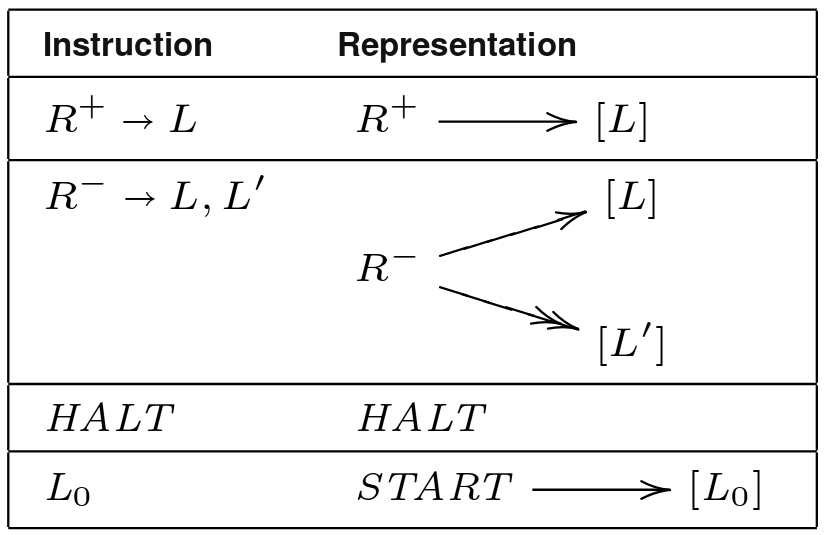
\includegraphics[width=0.45\columnwidth]{img/rm-representation} 
\end{table}

\paragraph{Configuration}

$\left(l,r_{0},\dots,r_{n}\right)$, where $l$ is the current label
and $r_{k}$ is the contents of $R_{k}$.

\paragraph{Computation}

Sequence of configurations. 
\begin{itemize}
\item \emph{Halting computation}: Computation where the last configuration
$c_{m}=\left(l,\dots\right)$ is halting configuration: 
\begin{itemize}
\item \emph{Proper halt}: $L_{l}$ is $HALT$. 
\item \emph{Erroneous halt}: Jumps to an instruction that doesn't exist. 
\end{itemize}
\item Computation is \emph{deterministic}: relation between initial and
final register contents is a \emph{partial function}. 
\end{itemize}

\subsection{Computable Functions}

\paragraph{Definition}

$f\in\mathbb{N}^{n}\rightharpoonup\mathbb{N}$ is computable if there
is a register machine $M$ such that for all $\left(x_{1},\dots,x_{n}\right)\in\mathbb{N}^{n}$
and all $y\in\mathbb{N}$: 
\begin{quotation}
The computation of $M$ starting with $R_{0}=0,R_{1}=x_{1},\dots,R_{n}=x_{n}$
and all other registers set to 0, halts with $R_{0}=y$ if and only
if $f\left(x_{1},\dots,x_{n}\right)=y$. 
\end{quotation}

\paragraph{Halting Problem}
\begin{itemize}
\item $S$ is a set of pairs $\left(A,D\right)$ where $A$ is an algorithm
and $D$ is some datum on which it operates. 
\item $A\left(D\right)\downarrow$ holds for $\left(A,D\right)\in S$ if
algorithm $A$ applied to $D$ halts. 
\end{itemize}
The Church-Truing thesis shows that there is no algorithm $H$ s.t.
for all $\left(A,D\right)\in S$: 
\[
H\left(A,D\right)=\begin{cases}
1 & A\left(D\right)\downarrow\\
0 & \text{otherwise}
\end{cases}
\]

\paragraph{G�del Numberings}

We code pairs numerically: 
\begin{itemize}
\item $\llangle x,y\rrangle\triangleq2^{x}\left(2y+1\right)$. 
\item $\left\langle x,y\right\rangle \triangleq2^{x}\left(2y+1\right)-1$. 
\end{itemize}
We code lists numerically: 
\begin{itemize}
\item $\ulcorner[]\urcorner\triangleq0$. 
\item $\ulcorner x::l\urcorner\triangleq\llangle x,\ulcorner l\urcorner\rrangle=2^{x}\left(2\times\ulcorner l\urcorner+1\right)$. 
\end{itemize}
We code programs numerically: 
\begin{itemize}
\item $\ulcorner P\urcorner\triangleq\ulcorner\left[\ulcorner\text{body}_{0}\urcorner,\dots,\ulcorner\text{body}_{n}\urcorner\right]\urcorner$. 
\end{itemize}
where instruction bodies are coded: 
\begin{itemize}
\item $\ulcorner R_{i}^{+}\rightarrow L_{j}\urcorner\triangleq\llangle2i,j\rrangle$ 
\item $\ulcorner R_{i}^{-}\rightarrow L_{j},L_{k}\urcorner\triangleq\llangle2i+1,\left\langle j,k\right\rangle \rrangle$ 
\item $\ulcorner HALT\urcorner\triangleq0$. 
\end{itemize}

\subsection{Gadgets}

\subsubsection*{Zero $R_{0}$}

\begin{figure}[H]
\centering{}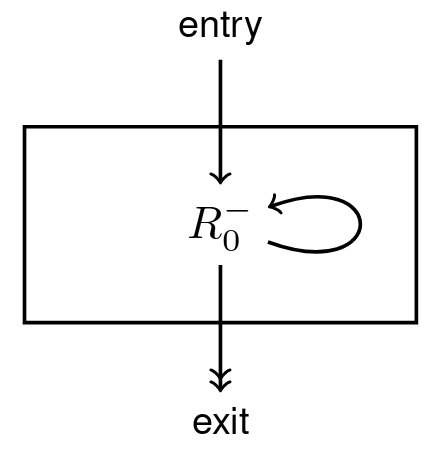
\includegraphics[width=0.3\columnwidth]{img/zero} 
\end{figure}

\subsubsection*{Add $R_{1}$ to $R_{2}$}

\begin{figure}[H]
\centering{}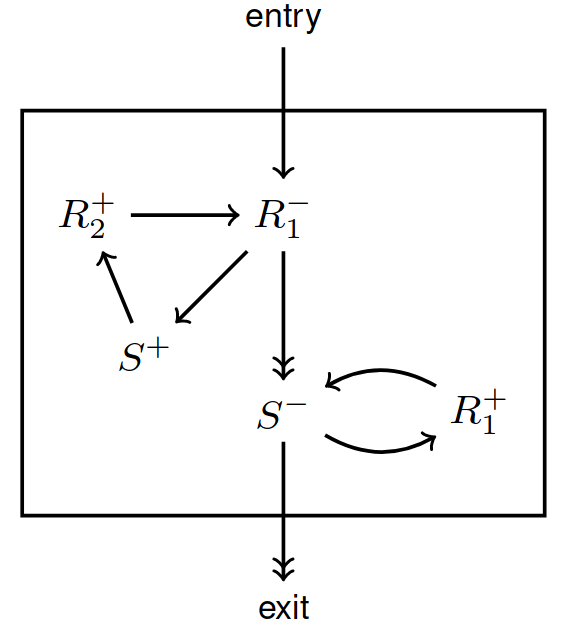
\includegraphics[width=0.4\columnwidth]{img/add} 
\end{figure}

\subsubsection*{Multiply $R_{1}$ by $R_{2}$ to $R_{0}$}

\begin{figure}[H]
\centering{}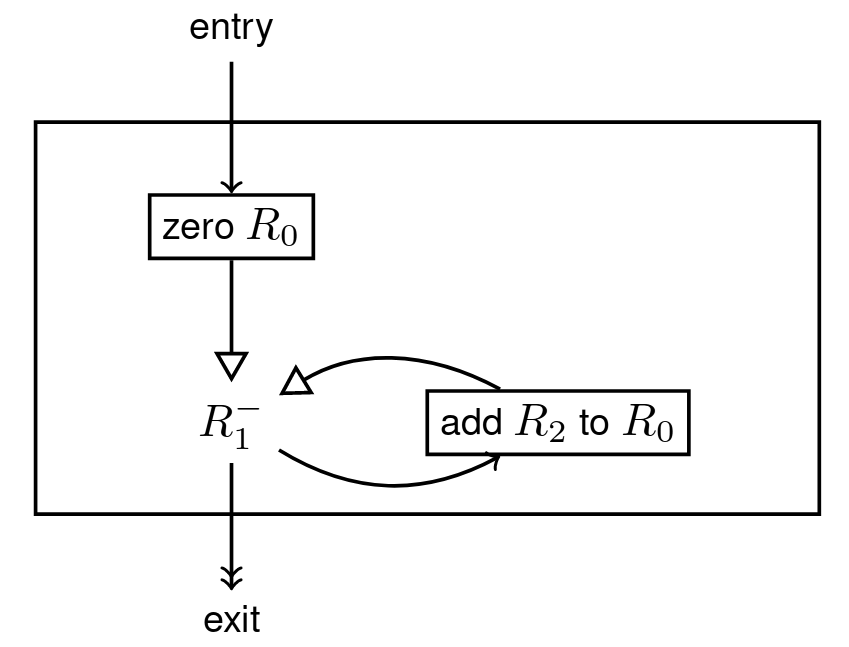
\includegraphics[width=0.6\columnwidth]{img/mult} 
\end{figure}

\subsubsection{Reasoning about Gadgets}
\begin{itemize}
\item Test it on various inputs and look for patterns. 
\item Break up into bits we understand. 
\item Use invariants. 
\begin{itemize}
\item Write out \emph{verification conditions}: conditions, in terms of
invariants and changes, for which an invariant must hold. 
\item Start out with $\bot$ and weaken the invariant until a pattern emerges. 
\end{itemize}
\end{itemize}

\subsubsection*{Push $X$ to $L$}

\begin{figure}[H]
\centering{}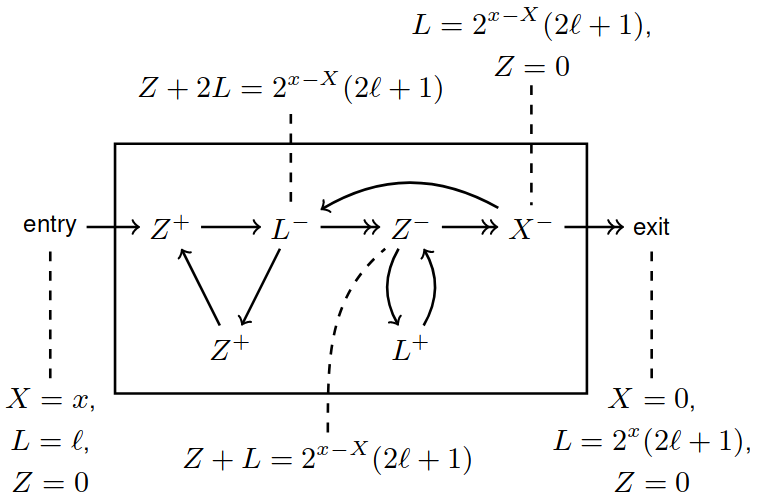
\includegraphics[width=0.65\columnwidth]{img/push} 
\end{figure}

\subsubsection*{Pop $L$ to $X$}

\begin{figure}[H]
\centering{}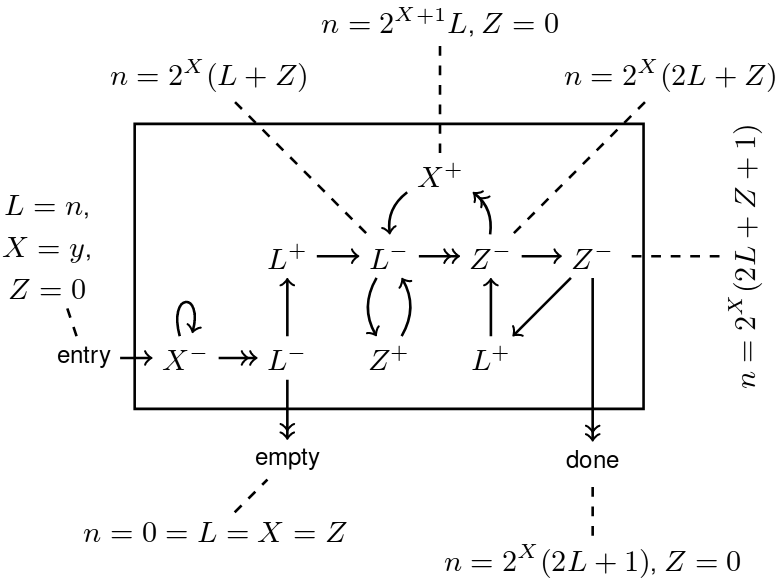
\includegraphics[width=0.675\columnwidth]{img/pop} 
\end{figure}

\subsection{Universal Register Machine}

Simulates an arbitrary register machine on arbitrary input. 
\begin{enumerate}
\item Copy the $PC$th item of $P$ to $N$. 
\item If $N=0$ halt, else decode $N$ as $\llangle y,z\rrangle$. Set $C::=y$
and $N::=z$. 
\item Copy the $i$th item of list $A$ into $R$ (where $C=2i$ or $2i+1$). 
\item Execute the current instruction on $R$, update $PC$ to next label,
and restore register value to $A$. 
\end{enumerate}

\subsection{Halting Problem for Register Machines}

$H$ decides the problem if given: 
\begin{itemize}
\item $R_{0}=0$. 
\item $R_{1}=e$. 
\item $R_{2}=\ulcorner\left[a_{1},\dots,a_{n}\right]\urcorner$ 
\end{itemize}
$H$ always halts with $R_{0}$ equal to 0 or 1. $R_{0}=1$ iff the
program represented by $e$ eventually halts when started with $R_{0}=0,\dots,R_{n}=a_{n}$
and all other registers zeroed.

\paragraph{Proof that $H$ Cannot Exist}
\begin{itemize}
\item Consider $H'=H$ with $R_{1}$ pushed onto $R_{2}$. 
\item Consider $C=H'$ where $C$ halts iff $H'$ halts with $R_{0}=0$. 
\end{itemize}
Assume $H$ exists:

\begin{multline*}
C\text{ started with }R_{1}=c\text{ halts}\\
\iff H'\text{ started with }R_{1}=c\text{ halts with }R_{0}=0\\
\iff H\text{ started with }R_{1}=c,R_{2}=\ulcorner\left[c\right]\urcorner\text{ halts with }R_{0}=0\\
\iff\text{prog}\left(c\right)\text{ started with }R_{1}=c\text{ does not halt}\\
\iff C\text{ started with }R_{1}=c\text{ does not halt}
\end{multline*}

Contradiction!

\section{Lambda Calculus}

\subsection{Syntax of the $\lambda$-Calculus}

\paragraph{$\lambda$-Terms}

\[
M::=x\mid\lambda x.M\mid MM
\]
\begin{itemize}
\item $\lambda x.M$ is a \emph{$\lambda$-abstraction}. 
\item $MM$ is an \emph{application}. 
\item $\lambda x.xy$ means $\lambda x.\left(xy\right)$. 
\item $\lambda x_{1}\dots x_{n}.M$ means $\lambda x_{1}.\left(\dots\left(\lambda x_{n}.M\right)\dots\right)$. 
\item $M_{1}M_{2}\dots M_{n}$ means $\left(\dots\left(M_{1}M_{2}\right)\dots\right)M_{n}$. 
\end{itemize}

\paragraph{Free and Bound Variables}
\begin{itemize}
\item \emph{Binding} occurrence if $x$ is between $\lambda$ and $.$. 
\item \emph{Bound} if in the body of a binding occurrence of $x$. 
\item \emph{Free} if neither binding nor bound. 
\end{itemize}
The set of free variables $FV\left(M\right)$ is calculated by: 
\begin{itemize}
\item $FV\left(x\right)=\left\{ x\right\} $. 
\item $FV\left(\lambda x.M\right)=FV\left(M\right)-\left\{ x\right\} $. 
\item $FV\left(MN\right)=FV\left(M\right)\cup FV\left(N\right)$. 
\end{itemize}
If $FV\left(M\right)=\emptyset$, $M$ is a \emph{closed term} / \emph{combinator}.

\paragraph{Substitution}
\begin{itemize}
\item $x\left[M/y\right]=\begin{cases}
M & x=y\\
x & x\neq y
\end{cases}$ 
\item $\left(\lambda x.N\right)\left[M/y\right]=\begin{cases}
\lambda x.N & x=y\\
\lambda z.N\left[z/x\right]\left[M/y\right] & x\neq y
\end{cases}$ 
\item $\left(M_{1}M_{2}\right)\left[M/y\right]=\left(M_{1}\left[M/y\right]\right)\left(M_{2}\left[M/y\right]\right)$ 
\end{itemize}

\paragraph{$\alpha$-Equivalence}
\begin{itemize}
\item $\begin{array}{c}
\\
\hline x=_{\alpha}x
\end{array}$. 
\item $\begin{array}{c}
M\left[z/x\right]=_{\alpha}N\left[z/y\right]\qquad z\notin FV\left(M\right)\cup FV\left(N\right)\\
\hline \lambda x.M=_{\alpha}\lambda y.N
\end{array}$. 
\item $\begin{array}{c}
M=_{\alpha}M'\qquad N=_{\alpha}N'\\
\hline MN=_{\alpha}M'N'
\end{array}$. 
\end{itemize}

\subsection{Semantics of the $\lambda$-Calculus}

\paragraph{$\beta$-reduction}
\begin{itemize}
\item $\begin{array}{c}
\\
\hline \left(\lambda x.M\right)N\rightarrow_{\beta}M\left[N/x\right]
\end{array}$. 
\item $\begin{array}{c}
M\rightarrow_{\beta}M'\\
\hline \lambda x.M\rightarrow_{\beta}\lambda x.M'
\end{array}$. 
\item $\begin{array}{c}
M\rightarrow_{\beta}M'\\
\hline MN\rightarrow_{\beta}M'N
\end{array}$. 
\item $\begin{array}{c}
N\rightarrow_{\beta}N'\\
\hline MN\rightarrow_{\beta}MN'
\end{array}$. 
\item $\begin{array}{c}
N=_{\alpha}M\qquad M\rightarrow_{\beta}M'\qquad M'=_{\alpha}N'\\
\hline N\rightarrow_{\beta}N'
\end{array}$. 
\end{itemize}

\paragraph{Reflexive Transitive Closure of $\rightarrow_{\beta}$}
\begin{itemize}
\item $\begin{array}{c}
M=_{\alpha}M'\\
\hline M\rightarrow_{\beta}^{*}M'
\end{array}$. 
\item $\begin{array}{c}
M\rightarrow_{\beta}M''\qquad M''\rightarrow_{\beta}^{*}M'\\
\hline M\rightarrow_{\beta}^{*}M'
\end{array}$. 
\end{itemize}

\paragraph{Church-Rosser Theorem}

$\rightarrow_{\beta}^{*}$ is \emph{confluent}. 
\begin{quotation}
If $M\rightarrow_{\beta}^{*}M_{1}$ and $M\rightarrow_{\beta}^{*}M_{2}$
then there exists $M'$ such that

$M_{1}\rightarrow_{\beta}^{*}M'$ and $M_{2}\rightarrow_{\beta}^{*}M'$. 
\end{quotation}

\paragraph{$\beta$-Equivalence}

$M_{1}=_{\beta}M_{2}$ iff there exists $M$ such that $M_{1}\rightarrow_{\beta}^{*}M$
and $M_{2}\rightarrow_{\beta}^{*}M$.

\paragraph{$\beta$-Normal Form}

A $\lambda$-term with no $\beta$-redexes. 
\begin{itemize}
\item $\beta$-normal forms are unique. 
\item Some $\lambda$-terms have no $\beta$-normal form. E.g. $\left(\lambda x.xx\right)\left(\lambda x.xx\right)$. 
\item Some $\lambda$-terms a $\beta$-normal form and also infinite chains
of reudction. E.g. $\left(\lambda x.y\right)\left(\lambda x.xx\right)\left(\lambda x.xx\right)$. 
\end{itemize}

\paragraph{$\lambda$-Definable Functions}
\begin{itemize}
\item $f\in\mathbb{N}^{n}\rightharpoonup\mathbb{N}$ is $\lambda$-definable
if there is a closed $\lambda$-term $F$ that represents it, such
that: 
\begin{itemize}
\item If $f\left(x_{1},\dots,x_{n}\right)=y$ then $Fx_{1}\dots x_{n}=_{\beta}y$. 
\item If $f\left(x_{1},\dots,x_{n}\right)\uparrow$ then $Fx_{1}\dots x_{n}$
has no $\beta$-normal form. 
\end{itemize}
\item A function is computable iff it is $\lambda$-definable. 
\end{itemize}

\end{document}
